\documentclass[10pt]{jarticle}
\usepackage[dvipdfmx]{graphicx}
\usepackage{amsmath}
\usepackage{comment}
\usepackage{setspace}
\usepackage{float}
\usepackage{indentfirst}
\usepackage{here}
\usepackage{caption}
\usepackage{multicol}

\captionsetup[figure]{font=footnotesize}

\setlength{\hoffset}{0cm}
\setlength{\oddsidemargin}{-15mm}
\setlength{\evensidemargin}{-3cm}
\setlength{\marginparsep}{0cm}
\setlength{\marginparwidth}{0cm}
\setlength{\textheight}{26.7cm}
\setlength{\textwidth}{19cm}
\setlength{\topmargin}{-50pt}      % 上の余白を調整
\setlength\abovecaptionskip{0pt}

\renewcommand{\baselinestretch}{1.0}
\renewcommand{\floatpagefraction}{1}
\renewcommand{\topfraction}{1}
\renewcommand{\bottomfraction}{1}
\renewcommand{\textfraction}{0}
\renewcommand{\labelenumi}{(\arabic{enumi})}
\renewcommand{\figurename}{Fig.} %図をFig.にする(画像のとこだけ)

\begin{comment}
  %図のキャプションからコロン:を消す
  \makeatletter
  \long\def\@makecaption#1#2{% #1=図表番号,#2=キャプション本文
    \sbox\@tempboxa{#1. #2}
    \ifdim \wd\@tempboxa >\hsize
    #1 #2\par 
    \else
    \hb@xt@\hsize{\hfil\box\@tempboxa\hfil}
    \fi
  }  
  \makeatother 
\end{comment}

%%sectionの前後の余白を消す
\makeatletter
\def\section{\@startsection {section}{1}{\z@}{-0.5ex plus -1ex minus -.2ex}{0.5 ex plus .2ex}{\small\bf}}
\def\subsection{\@startsection {subsection}{1}{\z@}{-0.5ex plus -1ex minus -.2ex}{0.5 ex plus .2ex}{\small\bf}}
\def\subsubsection{\@startsection {subsubsection}{1}{\z@}{-0.5ex plus -1ex minus -.2ex}{0.5 ex plus .2ex}{\footnotesize\bf}}
\makeatother

\pagestyle{myheadings}
%\pagestyle{empty} % すべてのページ番号を消去

\begin{document}
%文字サイズ
%\scriptsize   %7pt
\footnotesize %8pt
%\small        %9pt

\markright{第 16 回全日本学生フォーミュラ大会 Car No.029 九州工業大学デザインレポート}
%%\multicolumn{1}{|c|}{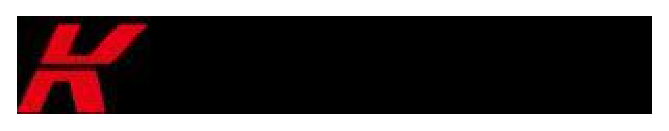
\includegraphics[width=10mm]{figure/eps/Logo.eps}}

%% \markleft{
%%   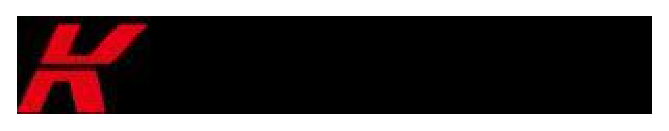
\includegraphics[width=10mm]{figure/eps/Logo.eps}
%% }

\date{\vspace{-15mm}}
\title{\vspace{-18mm} \small Car No.029 Kyushu Institute of Technology KIT-formula Design Report}

\oddsidemargin = -15mm
\maketitle % 実際の表題の出力
\thispagestyle{empty}
%\tableofcontents

%タイトル
%% \begin{center}
%%   {ji}
%% \end{center}


%\newpage
%イントロ
昨年度のKIT-formulaでは,2017年度大会において総合32位という結果に終わり,目標としていた歴代最高順位の8位を超える6位入賞を達成することが出来なかった.
したがって今年度では,根本的な車両の成り立ちを見直し,昨年度車両(以下KS-14)よりも確実に速く,勝てる車両を目指した.
そこで今年度の車両コンセプトを,昨年度よりも数段速い車両を意味し,また新たなことに挑戦するというチームの想いを込めた「Speed Evolution」とし,シングルナンバー(総合順位一桁)を目標に今年度車両(以下KS-15)の開発を行った.


\begin{multicols}{2}
%コンセプト
%%%%%%%%%%%%%%%%%%%%%%%%%%%
\section{車両開発方針}
%%%%%%%%%%%%%%%%%%%%%%%%%%%
車両開発の目標であるシングルナンバーを獲得するため,動的競技のうち最も総合順位との相関のあるエンデュランスに着目した.過去3年の大会結果から,総合順位一桁のチームはエンデュランスにおいても高順位であることが分かった.そこで昨年度の結果から,エンデュランス総合タイムが1320 sec(平均タイム66.0 sec/lap)で総合順位が8位以上を獲得できることが分かったため,これを車両開発目標に設定し開発を行った.

%%%%%%%%%%%%%%%%%%%%%%%%%%%
\subsection{ベンチマーク分析}
%%%%%%%%%%%%%%%%%%%%%%%%%%%
前項にて設定したエンデュランス総合タイムで走行していた2017年度大会の他大学車両と,KS-14との間でどういった区間でタイム差が生じているかをベンチマークとして,昨年度大会の動画から検証を行った.動画から区間A,Bを設定し(区間A:高速状態での加速性能,旋回性能が重視される区間,区間B:低速からの加速性能,応答性能が重視される区間)分析を行ったところ,区間Aでは平均して$\Delta$1.557 sec,区間Bでは$\Delta$2.379 secと,KS-14とベンチマークとの間に差があることが分かった.そこでパワートレインでは主にエンジン低回転領域からの加速性能,サスペンションでは旋回性能に加え応答性能を重視して開発を行った.またフレームやエアロデバイスといったボディではサスペンションの性能要求を満たすこと,コクピットにおいては従来のDrivabilityに加え,今まで重要視していなかったドライバーの快適性(以下Comfortability)を追求することとした.またサスペンションからの性能要求を満たすため,各パーツにおいて軽量化の検討を行った.


%サスペンション
%%%%%%%%%%%%%%%%%%%%%%%%%%%
\section{サスペンション}
%%%%%%%%%%%%%%%%%%%%%%%%%%%
チーム目標であるシングルナンバーを獲得するためにサスペンション系では前述のコース,タイム分析からコーナーの定常領域で0.54 sec,過渡領域であるパイロンスラロームにおいて1.84 secの短縮が必要であることが分かった.

%suspension
%%%%%%%%%%%%%%%%%%%%%%%%%%%
\subsection{subtitle}
%%%%%%%%%%%%%%%%%%%%%%%%%%%
あいうえお(Fig.\ref{fig:label1}).

かきくけこ(Fig.\ref{fig:label2}).



%hubs
%%%%%%%%%%%%%%%%%%%%%%%%%%%
\section{title}
%%%%%%%%%%%%%%%%%%%%%%%%%%%
aaaaaaaaaaaaaa

%%%%%%%%%%%%%%%%%%%%%%%%%%%
\subsection{subtitle}
%%%%%%%%%%%%%%%%%%%%%%%%%%%
bbbbbbbbbbbbbb

%%%%%%%%%%%%%%%%%%%%%%%%%%%
\subsubsection{subsubtitle}
%%%%%%%%%%%%%%%%%%%%%%%%%%%
cccccccccccccc


%uplights
%%%%%%%%%%%%%%%%%%%%%%%%%%%
\section{title}
%%%%%%%%%%%%%%%%%%%%%%%%%%%
aaaaaaaaaaaaaa

%%%%%%%%%%%%%%%%%%%%%%%%%%%
\subsection{subtitle}
%%%%%%%%%%%%%%%%%%%%%%%%%%%
bbbbbbbbbbbbbb

%%%%%%%%%%%%%%%%%%%%%%%%%%%
\subsubsection{subsubtitle}
%%%%%%%%%%%%%%%%%%%%%%%%%%%
cccccccccccccc



%ボディ
%%%%%%%%%%%%%%%%%%%%%%%%%%%
\section{ボディ}
%%%%%%%%%%%%%%%%%%%%%%%%%%%
aaaaaaaaaaaaaaaaaaaaaaaa

%ボディ
%%%%%%%%%%%%%%%%%%%%%%%%%%%
\section{title}
%%%%%%%%%%%%%%%%%%%%%%%%%%%
aaaaaaaaaaaaaa

%%%%%%%%%%%%%%%%%%%%%%%%%%%
\subsection{subtitle}
%%%%%%%%%%%%%%%%%%%%%%%%%%%
bbbbbbbbbbbbbb

%%%%%%%%%%%%%%%%%%%%%%%%%%%
\subsubsection{subsubtitle}
%%%%%%%%%%%%%%%%%%%%%%%%%%%
cccccccccccccc


%エアロ
%%%%%%%%%%%%%%%%%%%%%%%%%%%
\section{title}
%%%%%%%%%%%%%%%%%%%%%%%%%%%
aaaaaaaaaaaaaa

%%%%%%%%%%%%%%%%%%%%%%%%%%%
\subsection{subtitle}
%%%%%%%%%%%%%%%%%%%%%%%%%%%
bbbbbbbbbbbbbb

%%%%%%%%%%%%%%%%%%%%%%%%%%%
\subsubsection{subsubtitle}
%%%%%%%%%%%%%%%%%%%%%%%%%%%
cccccccccccccc



%パワートレイン
%%%%%%%%%%%%%%%%%%%%%%%%%%%
\section{ボディ}
%%%%%%%%%%%%%%%%%%%%%%%%%%%
aaaaaaaaaaaaaaaaaaaaaaaa

%ボディ
%%%%%%%%%%%%%%%%%%%%%%%%%%%
\section{title}
%%%%%%%%%%%%%%%%%%%%%%%%%%%
aaaaaaaaaaaaaa

%%%%%%%%%%%%%%%%%%%%%%%%%%%
\subsection{subtitle}
%%%%%%%%%%%%%%%%%%%%%%%%%%%
bbbbbbbbbbbbbb

%%%%%%%%%%%%%%%%%%%%%%%%%%%
\subsubsection{subsubtitle}
%%%%%%%%%%%%%%%%%%%%%%%%%%%
cccccccccccccc


%エアロ
%%%%%%%%%%%%%%%%%%%%%%%%%%%
\section{title}
%%%%%%%%%%%%%%%%%%%%%%%%%%%
aaaaaaaaaaaaaa

%%%%%%%%%%%%%%%%%%%%%%%%%%%
\subsection{subtitle}
%%%%%%%%%%%%%%%%%%%%%%%%%%%
bbbbbbbbbbbbbb

%%%%%%%%%%%%%%%%%%%%%%%%%%%
\subsubsection{subsubtitle}
%%%%%%%%%%%%%%%%%%%%%%%%%%%
cccccccccccccc



%エルゴノミクス
%%%%%%%%%%%%%%%%%%%%%%%%%%%
\section{コクピット・コントロール}
%%%%%%%%%%%%%%%%%%%%%%%%%%%
従来までは主にDrivabilityの向上をコクピットの目標としていた.しかしKS-14では,シートのホールド性やステアリングを切った際のドライバーの肘と足の干渉など,操作以前にドライビングに不快感を与える要素が存在していた.したがってKS-15ではDrivabilityの向上に加えComfortabilityを重視した開発を行った.

%シフター
%%%%%%%%%%%%%%%%%%%%%%%%%%%
\section{title}
%%%%%%%%%%%%%%%%%%%%%%%%%%%
aaaaaaaaaaaaaa

%%%%%%%%%%%%%%%%%%%%%%%%%%%
\subsection{subtitle}
%%%%%%%%%%%%%%%%%%%%%%%%%%%
bbbbbbbbbbbbbb

%%%%%%%%%%%%%%%%%%%%%%%%%%%
\subsubsection{subsubtitle}
%%%%%%%%%%%%%%%%%%%%%%%%%%%
cccccccccccccc


%ペダル
%%%%%%%%%%%%%%%%%%%%%%%%%%%
\section{title}
%%%%%%%%%%%%%%%%%%%%%%%%%%%
aaaaaaaaaaaaaa

%%%%%%%%%%%%%%%%%%%%%%%%%%%
\subsection{subtitle}
%%%%%%%%%%%%%%%%%%%%%%%%%%%
bbbbbbbbbbbbbb

%%%%%%%%%%%%%%%%%%%%%%%%%%%
\subsubsection{subsubtitle}
%%%%%%%%%%%%%%%%%%%%%%%%%%%
cccccccccccccc


%スロットル
%%%%%%%%%%%%%%%%%%%%%%%%%%%
\section{title}
%%%%%%%%%%%%%%%%%%%%%%%%%%%
aaaaaaaaaaaaaa

%%%%%%%%%%%%%%%%%%%%%%%%%%%
\subsection{subtitle}
%%%%%%%%%%%%%%%%%%%%%%%%%%%
bbbbbbbbbbbbbb

%%%%%%%%%%%%%%%%%%%%%%%%%%%
\subsubsection{subsubtitle}
%%%%%%%%%%%%%%%%%%%%%%%%%%%
cccccccccccccc


%ステアリング
%%%%%%%%%%%%%%%%%%%%%%%%%%%
\section{title}
%%%%%%%%%%%%%%%%%%%%%%%%%%%
aaaaaaaaaaaaaa

%%%%%%%%%%%%%%%%%%%%%%%%%%%
\subsection{subtitle}
%%%%%%%%%%%%%%%%%%%%%%%%%%%
bbbbbbbbbbbbbb

%%%%%%%%%%%%%%%%%%%%%%%%%%%
\subsubsection{subsubtitle}
%%%%%%%%%%%%%%%%%%%%%%%%%%%
cccccccccccccc


%シート
%%%%%%%%%%%%%%%%%%%%%%%%%%%
\section{title}
%%%%%%%%%%%%%%%%%%%%%%%%%%%
aaaaaaaaaaaaaa

%%%%%%%%%%%%%%%%%%%%%%%%%%%
\subsection{subtitle}
%%%%%%%%%%%%%%%%%%%%%%%%%%%
bbbbbbbbbbbbbb

%%%%%%%%%%%%%%%%%%%%%%%%%%%
\subsubsection{subsubtitle}
%%%%%%%%%%%%%%%%%%%%%%%%%%%
cccccccccccccc



%参考文献
\begin{thebibliography}{99}
  \addcontentsline{toc}{section}{参考文献}
\bibitem{NACA} NATIONAL ADVISORY COMMITTEE FOR AERONAUTICS,"AERODYNAMIC CHARACTERISTICS OF AIRFOILS-IV",p.196,1926.
\end{thebibliography}

\end{multicols}


\clearpage
%図
\begin{figure}[H]
  \begin{tabular}{cccc}
    \begin{minipage}{0.24\hsize}
      \begin{center}
        \includegraphics[clip,width=3.5cm]{figure/susp/graph1.eps}
        \caption{エンデュランスとスキッドパッドの相関図}
        \label{fig:sus1}
      \end{center}
    \end{minipage}
    
    \begin{minipage}{0.24\hsize}
      \begin{center}
        \includegraphics[clip,width=3.5cm]{figure/susp/graph2.eps}
        \caption{車両重量のスキッドパッドへの影響}
        \label{fig:sus2}
      \end{center}
    \end{minipage}
    
    \begin{minipage}{0.24\hsize}
      \begin{center}
      \includegraphics[clip,width=3.5cm]{figure/susp/graph3.eps}
      \caption{ダウンフォースのスキッドパッドへの影響}
      \label{fig:sus3}
      \end{center}
    \end{minipage}
    
    \begin{minipage}{0.24\hsize}
      \begin{center}
        \includegraphics[clip,width=3.5cm]{figure/susp/graph4.eps}
        \caption{トレッドのスキッドパッドへの影響}
        \label{fig:sus4}
      \end{center}
    \end{minipage}
  \end{tabular}
\end{figure}  

\begin{figure}[H]
  \begin{tabular}{cccc}
    \begin{minipage}{0.24\hsize}
      \begin{center}
        \includegraphics[clip,width=3.5cm]{figure/susp/graph5.eps}
        \caption{軽量化とDF目標}
        \label{fig:sus5}
      \end{center}
    \end{minipage}
    
    \begin{minipage}{0.24\hsize}
      \begin{center}
        \includegraphics[clip,width=3.5cm]{figure/susp/graph6.eps}
        \caption{各校のホイールベースとタイム}
        \label{fig:sus6}
      \end{center}
    \end{minipage}

    \begin{minipage}{0.24\hsize}
      \begin{center}
        \includegraphics[clip,width=3.5cm]{figure/susp/graphA.eps}
        \caption{旋回外輪側キャンバーチェンジ}
        \label{fig:susA}
      \end{center}
    \end{minipage}

    \begin{minipage}{0.24\hsize}
      \begin{center}
        \includegraphics[clip,width=3.5cm]{figure/susp/graphB.eps}
        \caption{旋回外輪側トーチェンジ}
        \label{fig:susB}
      \end{center}
    \end{minipage}
  \end{tabular}
\end{figure}  

\begin{figure}[H]
  \begin{tabular}{cccc}
    \begin{minipage}{0.24\hsize}
      \begin{center}
        \includegraphics[clip,width=3.5cm]{figure/susp/graphC.eps}
        \caption{スカッフ変化}
        \label{fig:susC}
      \end{center}
    \end{minipage}

    \begin{minipage}{0.24\hsize}
      \begin{center}
        \includegraphics[clip,width=3.5cm]{figure/susp/graphD.eps}
        \caption{重心高低下によるタイムへの影響}
        \label{fig:susD}
      \end{center}
    \end{minipage}

    %% \begin{minipage}{0.24\hsize}
    %%   \begin{center}
    %%     \includegraphics[clip,width=3.5cm]{figure/uplight/graph1.eps}
    %%     \caption{ナット緩み防止溝加工図}
    %%     \label{fig:uplight1}
    %%   \end{center}
    %% \end{minipage}
    
    %% \begin{minipage}{0.24\hsize}
    %%   \begin{center}
    %%     \includegraphics[clip,width=3.5cm]{figure/uplight/graph2.eps}
    %%     \caption{トラクションコントロールセンサステー}
    %%     \label{fig:uplight2}
    %%   \end{center}
    %% \end{minipage}

    \begin{minipage}{0.24\hsize}
      \begin{center}
        \includegraphics[clip,width=3.5cm]{figure/frame/graph1.eps}
        \caption{横Gと右側後輪のダンパーのストローク量}
        \label{fig:frame1}
      \end{center}
    \end{minipage}

    \begin{minipage}{0.24\hsize}
      \begin{center}
        \includegraphics[clip,width=3.5cm]{figure/aero/pontoon.eps}
        \caption{サイドポンツーン周辺の空気の流れ}
        \label{fig:pontoon}
      \end{center}
    \end{minipage}
  \end{tabular}
\end{figure}  

\begin{figure}[H]
  \begin{tabular}{cccc}    
    \begin{minipage}{0.24\hsize}
      \begin{center}
        \includegraphics[clip,width=3.5cm]{figure/aero/angle_data.eps}
        \caption{迎角変化によるパラメータの変化}
        \label{fig:angle_data}
      \end{center}
    \end{minipage}
    
    \begin{minipage}{0.24\hsize}
      \begin{center}
        \includegraphics[clip,width=3.5cm]{figure/aero/naca97-deg20.eps}
        \caption{迎角20degのときの乱流エネルギー}
        \label{fig:naca97_deg20}
      \end{center}
    \end{minipage}

    \begin{minipage}{0.24\hsize}
      \begin{center}
        \includegraphics[clip,width=3.5cm]{figure/aero/naca97-deg15-15-15.eps}
        \caption{スリットを設けたときの乱流エネルギー}
        \label{fig:naca97_151515}
      \end{center}
    \end{minipage}

    \begin{minipage}{0.24\hsize}
      \begin{center}
        \includegraphics[clip,width=3.5cm]{figure/aero/straight.eps}
        \caption{タフト法(アクセラレーション)}
        \label{fig:taft_acc}
      \end{center}
    \end{minipage}
  \end{tabular}
\end{figure}  

\begin{figure}[H]
  \begin{tabular}{cccc}      
    \begin{minipage}{0.24\hsize}
      \begin{center}
        \includegraphics[clip,width=3.5cm]{figure/aero/turn.eps}
        \caption{タフト法(スキッドパッド)}
        \label{fig:taft_skid}
      \end{center}
    \end{minipage}

    \begin{minipage}{0.24\hsize}
      \begin{center}
        \includegraphics[clip,width=3.5cm]{figure/powertrain_exhast/graph1.eps}
        \caption{バルブタイミング変更による影響}
        \label{fig:power1}
      \end{center}
    \end{minipage}

    \begin{minipage}{0.24\hsize}
      \begin{center}
        \includegraphics[clip,width=3.5cm]{figure/intake/graph1.eps}
        \caption{バタフライ径変更による吸気流量の比較}
        \label{fig:intake1}
      \end{center}
    \end{minipage}

    \begin{minipage}{0.24\hsize}
      \begin{center}
        \includegraphics[clip,width=3.5cm]{figure/intake/graph2.eps}
        \caption{吸気変更によるエンジン性能の比較}
        \label{fig:intake2}
      \end{center}
    \end{minipage}
  \end{tabular}
\end{figure}  

\begin{figure}[H]
  \begin{tabular}{cccc}
    \begin{minipage}{0.24\hsize}
      \begin{center}
        \includegraphics[clip,width=3.5cm]{figure/intake/graph3.eps}
        \caption{各気筒の吸気流量}
        \label{fig:intake3}
      \end{center}
    \end{minipage}

    %% \begin{minipage}{0.24\hsize}
    %%   \begin{center}
    %%     \includegraphics[clip,width=3.5cm]{figure/powertrain_exhast/graph2.eps}
    %%     \caption{排気管集合部の一体化}
    %%     \label{fig:power2}
    %%   \end{center}
    %% \end{minipage}

    \begin{minipage}{0.24\hsize}
      \begin{center}
        \includegraphics[clip,width=3.5cm]{figure/powertrain_exhast/graph3.eps}
        \caption{4つのA/Fセンサマウント}
        \label{fig:power3}
      \end{center}
    \end{minipage}
 
    \begin{minipage}{0.24\hsize}
      \begin{center}
        \includegraphics[clip,width=3.5cm]{figure/powertrain_exhast/graph4.eps}
        \caption{排気変更による特性の比較}
        \label{fig:power4}
      \end{center}
    \end{minipage}

    \begin{minipage}{0.24\hsize}
      \begin{center}
        \includegraphics[clip,width=3.5cm]{figure/powertrain_exhast/graph5.eps}
        \caption{チャンバー有無での騒音の比較}
        \label{fig:power5}
      \end{center}
    \end{minipage}
  \end{tabular}
\end{figure}  

\begin{figure}[H]
  \begin{tabular}{cccc}
    \begin{minipage}{0.24\hsize}
      \begin{center}
        \includegraphics[clip,width=3.5cm]{figure/powertrain_exhast/graph6.eps}
        \caption{サイレンサエンド部の長さ比較}
        \label{fig:power6}
      \end{center}
    \end{minipage}

    \begin{minipage}{0.24\hsize}
      \begin{center}
        \includegraphics[clip,width=3.5cm]{figure/radiator/graph1.eps}
        \caption{Radiator Layout\newline 上:KS-14,下:KS-15}
        \label{fig:radiator1}
      \end{center}
    \end{minipage}
    
    \begin{minipage}{0.24\hsize}
      \begin{center}
        \includegraphics[clip,width=3.5cm]{figure/fuel/graph1.eps}
        \caption{バッフルプレート\newline (該当箇所は色がついた部分)}
        \label{fig:fuel1}
      \end{center}
    \end{minipage}

    \begin{minipage}{0.24\hsize}
      \begin{center}
        \includegraphics[clip,width=3.5cm]{figure/fuel/graph2.eps}
        \caption{ANSYSによる解析結果}
        \label{fig:fuel2}
      \end{center}
    \end{minipage}
  \end{tabular}
\end{figure}

\end{document}
